

\begin{document}




\begin{document}




\begin{document}




\begin{document}


\include{giulia}
\begin{comment}
We should probably keep both since we have them, and compare the results saying something like "with more data and fewer features (due to the use of an atlas with 120 ROIs) we have better/worse performance than using the correlation matrices obtained with our C-PAC pipeline."
\end{comment}

In addition, we also repeated the steps that were supposedly taken by C-PAC in the generation of the correlation matrices (we can only guess as to how they were actually obtained due too lack of in depth documentation) to obtain the correlation matrices for all the processed fMRIs, since we realized that the C-PAC preprocessing script had at times failed to generate the ROI analysis output for some subjects. We followed the general indications of Kassraian-Fard et al.\cite{guidelinesml}. They recommended using a Craddock atlas, which is available to fetch from nilearn's\cite{10.3389/fninf.2014.00014} database, to identify the regions of interest. This atlas is not the same as the one used by C-PAC, because it's a 4D atlas instead of 3D, and it has 120 instead of 200 ROIs. For all those 120 ROIs, we compute the average time series and then the correlation matrix containing the correlation of each pair of time series. The result is a 120x120 symmetric matrix, which translates to 7140 unique features.

%% maybe in a different section:
We thought it could be interesting to compare the performance of the model with a different number of features, since we saw early on that our baseline model with 200 ROIs was overfitting heavily. 

\begin{figure}[h]
\caption{ROIs highlighted on Craddock atlas}
\centering
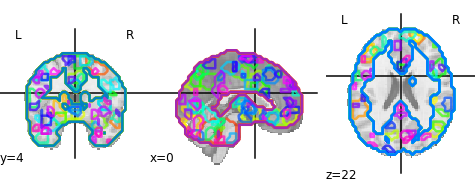
\includegraphics[width=0.75\textwidth]{final_report/atlas.png}
\end{figure}



\begin{comment}
NILEARN citation:

@ARTICLE{10.3389/fninf.2014.00014,
  
AUTHOR={Abraham, Alexandre and Pedregosa, Fabian and Eickenberg, Michael and Gervais, Philippe and Mueller, Andreas and Kossaifi, Jean and Gramfort, Alexandre and Thirion, Bertrand and Varoquaux, Gael},   
	 
TITLE={Machine learning for neuroimaging with scikit-learn},      
	
JOURNAL={Frontiers in Neuroinformatics},      
	
VOLUME={8},      
	
YEAR={2014},      
	  
URL={https://www.frontiersin.org/article/10.3389/fninf.2014.00014},       
	
DOI={10.3389/fninf.2014.00014},      
	
ISSN={1662-5196},   
   
ABSTRACT={Statistical machine learning methods are increasingly used for neuroimaging data analysis. Their main virtue is their ability to model high-dimensional datasets, e.g., multivariate analysis of activation images or resting-state time series. Supervised learning is typically used in decoding or encoding settings to relate brain images to behavioral or clinical observations, while unsupervised learning can uncover hidden structures in sets of images (e.g., resting state functional MRI) or find sub-populations in large cohorts. By considering different functional neuroimaging applications, we illustrate how scikit-learn, a Python machine learning library, can be used to perform some key analysis steps. Scikit-learn contains a very large set of statistical learning algorithms, both supervised and unsupervised, and its application to neuroimaging data provides a versatile tool to study the brain.}
}
\end{comment}
\end{document}

\begin{comment}
We should probably keep both since we have them, and compare the results saying something like "with more data and fewer features (due to the use of an atlas with 120 ROIs) we have better/worse performance than using the correlation matrices obtained with our C-PAC pipeline."
\end{comment}

In addition, we also repeated the steps that were supposedly taken by C-PAC in the generation of the correlation matrices (we can only guess as to how they were actually obtained due too lack of in depth documentation) to obtain the correlation matrices for all the processed fMRIs, since we realized that the C-PAC preprocessing script had at times failed to generate the ROI analysis output for some subjects. We followed the general indications of Kassraian-Fard et al.\cite{guidelinesml}. They recommended using a Craddock atlas, which is available to fetch from nilearn's\cite{10.3389/fninf.2014.00014} database, to identify the regions of interest. This atlas is not the same as the one used by C-PAC, because it's a 4D atlas instead of 3D, and it has 120 instead of 200 ROIs. For all those 120 ROIs, we compute the average time series and then the correlation matrix containing the correlation of each pair of time series. The result is a 120x120 symmetric matrix, which translates to 7140 unique features.

%% maybe in a different section:
We thought it could be interesting to compare the performance of the model with a different number of features, since we saw early on that our baseline model with 200 ROIs was overfitting heavily. 

\begin{figure}[h]
\caption{ROIs highlighted on Craddock atlas}
\centering
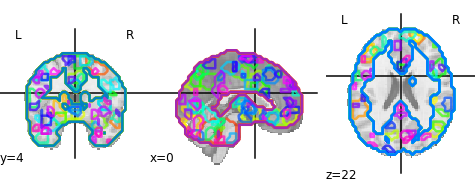
\includegraphics[width=0.75\textwidth]{final_report/atlas.png}
\end{figure}



\begin{comment}
NILEARN citation:

@ARTICLE{10.3389/fninf.2014.00014,
  
AUTHOR={Abraham, Alexandre and Pedregosa, Fabian and Eickenberg, Michael and Gervais, Philippe and Mueller, Andreas and Kossaifi, Jean and Gramfort, Alexandre and Thirion, Bertrand and Varoquaux, Gael},   
	 
TITLE={Machine learning for neuroimaging with scikit-learn},      
	
JOURNAL={Frontiers in Neuroinformatics},      
	
VOLUME={8},      
	
YEAR={2014},      
	  
URL={https://www.frontiersin.org/article/10.3389/fninf.2014.00014},       
	
DOI={10.3389/fninf.2014.00014},      
	
ISSN={1662-5196},   
   
ABSTRACT={Statistical machine learning methods are increasingly used for neuroimaging data analysis. Their main virtue is their ability to model high-dimensional datasets, e.g., multivariate analysis of activation images or resting-state time series. Supervised learning is typically used in decoding or encoding settings to relate brain images to behavioral or clinical observations, while unsupervised learning can uncover hidden structures in sets of images (e.g., resting state functional MRI) or find sub-populations in large cohorts. By considering different functional neuroimaging applications, we illustrate how scikit-learn, a Python machine learning library, can be used to perform some key analysis steps. Scikit-learn contains a very large set of statistical learning algorithms, both supervised and unsupervised, and its application to neuroimaging data provides a versatile tool to study the brain.}
}
\end{comment}
\end{document}

\begin{comment}
We should probably keep both since we have them, and compare the results saying something like "with more data and fewer features (due to the use of an atlas with 120 ROIs) we have better/worse performance than using the correlation matrices obtained with our C-PAC pipeline."
\end{comment}

In addition, we also repeated the steps that were supposedly taken by C-PAC in the generation of the correlation matrices (we can only guess as to how they were actually obtained due too lack of in depth documentation) to obtain the correlation matrices for all the processed fMRIs, since we realized that the C-PAC preprocessing script had at times failed to generate the ROI analysis output for some subjects. We followed the general indications of Kassraian-Fard et al.\cite{guidelinesml}. They recommended using a Craddock atlas, which is available to fetch from nilearn's\cite{10.3389/fninf.2014.00014} database, to identify the regions of interest. This atlas is not the same as the one used by C-PAC, because it's a 4D atlas instead of 3D, and it has 120 instead of 200 ROIs. For all those 120 ROIs, we compute the average time series and then the correlation matrix containing the correlation of each pair of time series. The result is a 120x120 symmetric matrix, which translates to 7140 unique features.

%% maybe in a different section:
We thought it could be interesting to compare the performance of the model with a different number of features, since we saw early on that our baseline model with 200 ROIs was overfitting heavily. 

\begin{figure}[h]
\caption{ROIs highlighted on Craddock atlas}
\centering
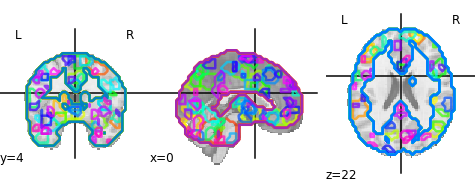
\includegraphics[width=0.75\textwidth]{final_report/atlas.png}
\end{figure}



\begin{comment}
NILEARN citation:

@ARTICLE{10.3389/fninf.2014.00014,
  
AUTHOR={Abraham, Alexandre and Pedregosa, Fabian and Eickenberg, Michael and Gervais, Philippe and Mueller, Andreas and Kossaifi, Jean and Gramfort, Alexandre and Thirion, Bertrand and Varoquaux, Gael},   
	 
TITLE={Machine learning for neuroimaging with scikit-learn},      
	
JOURNAL={Frontiers in Neuroinformatics},      
	
VOLUME={8},      
	
YEAR={2014},      
	  
URL={https://www.frontiersin.org/article/10.3389/fninf.2014.00014},       
	
DOI={10.3389/fninf.2014.00014},      
	
ISSN={1662-5196},   
   
ABSTRACT={Statistical machine learning methods are increasingly used for neuroimaging data analysis. Their main virtue is their ability to model high-dimensional datasets, e.g., multivariate analysis of activation images or resting-state time series. Supervised learning is typically used in decoding or encoding settings to relate brain images to behavioral or clinical observations, while unsupervised learning can uncover hidden structures in sets of images (e.g., resting state functional MRI) or find sub-populations in large cohorts. By considering different functional neuroimaging applications, we illustrate how scikit-learn, a Python machine learning library, can be used to perform some key analysis steps. Scikit-learn contains a very large set of statistical learning algorithms, both supervised and unsupervised, and its application to neuroimaging data provides a versatile tool to study the brain.}
}
\end{comment}
\end{document}

\begin{comment}
We should probably keep both since we have them, and compare the results saying something like "with more data and fewer features (due to the use of an atlas with 120 ROIs) we have better/worse performance than using the correlation matrices obtained with our C-PAC pipeline."
\end{comment}

In addition, we also repeated the steps that were supposedly taken by C-PAC in the generation of the correlation matrices (we can only guess as to how they were actually obtained due too lack of in depth documentation) to obtain the correlation matrices for all the processed fMRIs, since we realized that the C-PAC preprocessing script had at times failed to generate the ROI analysis output for some subjects. We followed the general indications of Kassraian-Fard et al.\cite{guidelinesml}. They recommended using a Craddock atlas, which is available to fetch from nilearn's\cite{10.3389/fninf.2014.00014} database, to identify the regions of interest. This atlas is not the same as the one used by C-PAC, because it's a 4D atlas instead of 3D, and it has 120 instead of 200 ROIs. For all those 120 ROIs, we compute the average time series and then the correlation matrix containing the correlation of each pair of time series. The result is a 120x120 symmetric matrix, which translates to 7140 unique features.

%% maybe in a different section:
We thought it could be interesting to compare the performance of the model with a different number of features, since we saw early on that our baseline model with 200 ROIs was overfitting heavily. 

\begin{figure}[h]
\caption{ROIs highlighted on Craddock atlas}
\centering
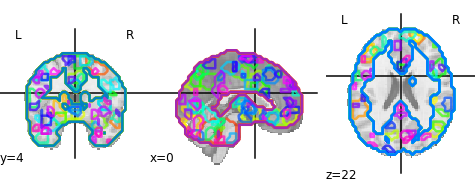
\includegraphics[width=0.75\textwidth]{final_report/atlas.png}
\end{figure}



\begin{comment}
NILEARN citation:

@ARTICLE{10.3389/fninf.2014.00014,
  
AUTHOR={Abraham, Alexandre and Pedregosa, Fabian and Eickenberg, Michael and Gervais, Philippe and Mueller, Andreas and Kossaifi, Jean and Gramfort, Alexandre and Thirion, Bertrand and Varoquaux, Gael},   
	 
TITLE={Machine learning for neuroimaging with scikit-learn},      
	
JOURNAL={Frontiers in Neuroinformatics},      
	
VOLUME={8},      
	
YEAR={2014},      
	  
URL={https://www.frontiersin.org/article/10.3389/fninf.2014.00014},       
	
DOI={10.3389/fninf.2014.00014},      
	
ISSN={1662-5196},   
   
ABSTRACT={Statistical machine learning methods are increasingly used for neuroimaging data analysis. Their main virtue is their ability to model high-dimensional datasets, e.g., multivariate analysis of activation images or resting-state time series. Supervised learning is typically used in decoding or encoding settings to relate brain images to behavioral or clinical observations, while unsupervised learning can uncover hidden structures in sets of images (e.g., resting state functional MRI) or find sub-populations in large cohorts. By considering different functional neuroimaging applications, we illustrate how scikit-learn, a Python machine learning library, can be used to perform some key analysis steps. Scikit-learn contains a very large set of statistical learning algorithms, both supervised and unsupervised, and its application to neuroimaging data provides a versatile tool to study the brain.}
}
\end{comment}
\end{document}
